
\documentclass[10pt]{report}
\usepackage[textwidth=17cm]{geometry}
\usepackage[utf8]{inputenc}
\usepackage[T1]{fontenc}
\usepackage{graphicx}

\begin{document}

    \begin{titlepage}
        \begin{center}

            \vspace*{\fill}
            \Huge
            \textbf{Projeto de Bases de Dados - Parte 1}
            
            \vspace*{\fill}

            \Large
            \textbf{Grupo 27} \\
            89427 - Daniel Seara - 33,3\% - 3 horas \\
            89399 - Afonso Gonçalves - 33,3\% - 3 horas \\
            89496 - Marcelo Santos - 33,3\% - 3 horas \\

            \bigskip
            \textbf{Turno:} 4ª Feira 9h30 - Lab 8\\ \textbf{Professor:} Duarte Galvão
        
        \end{center}
\end{titlepage}

\begin{center}
    \vspace*{-2cm}
    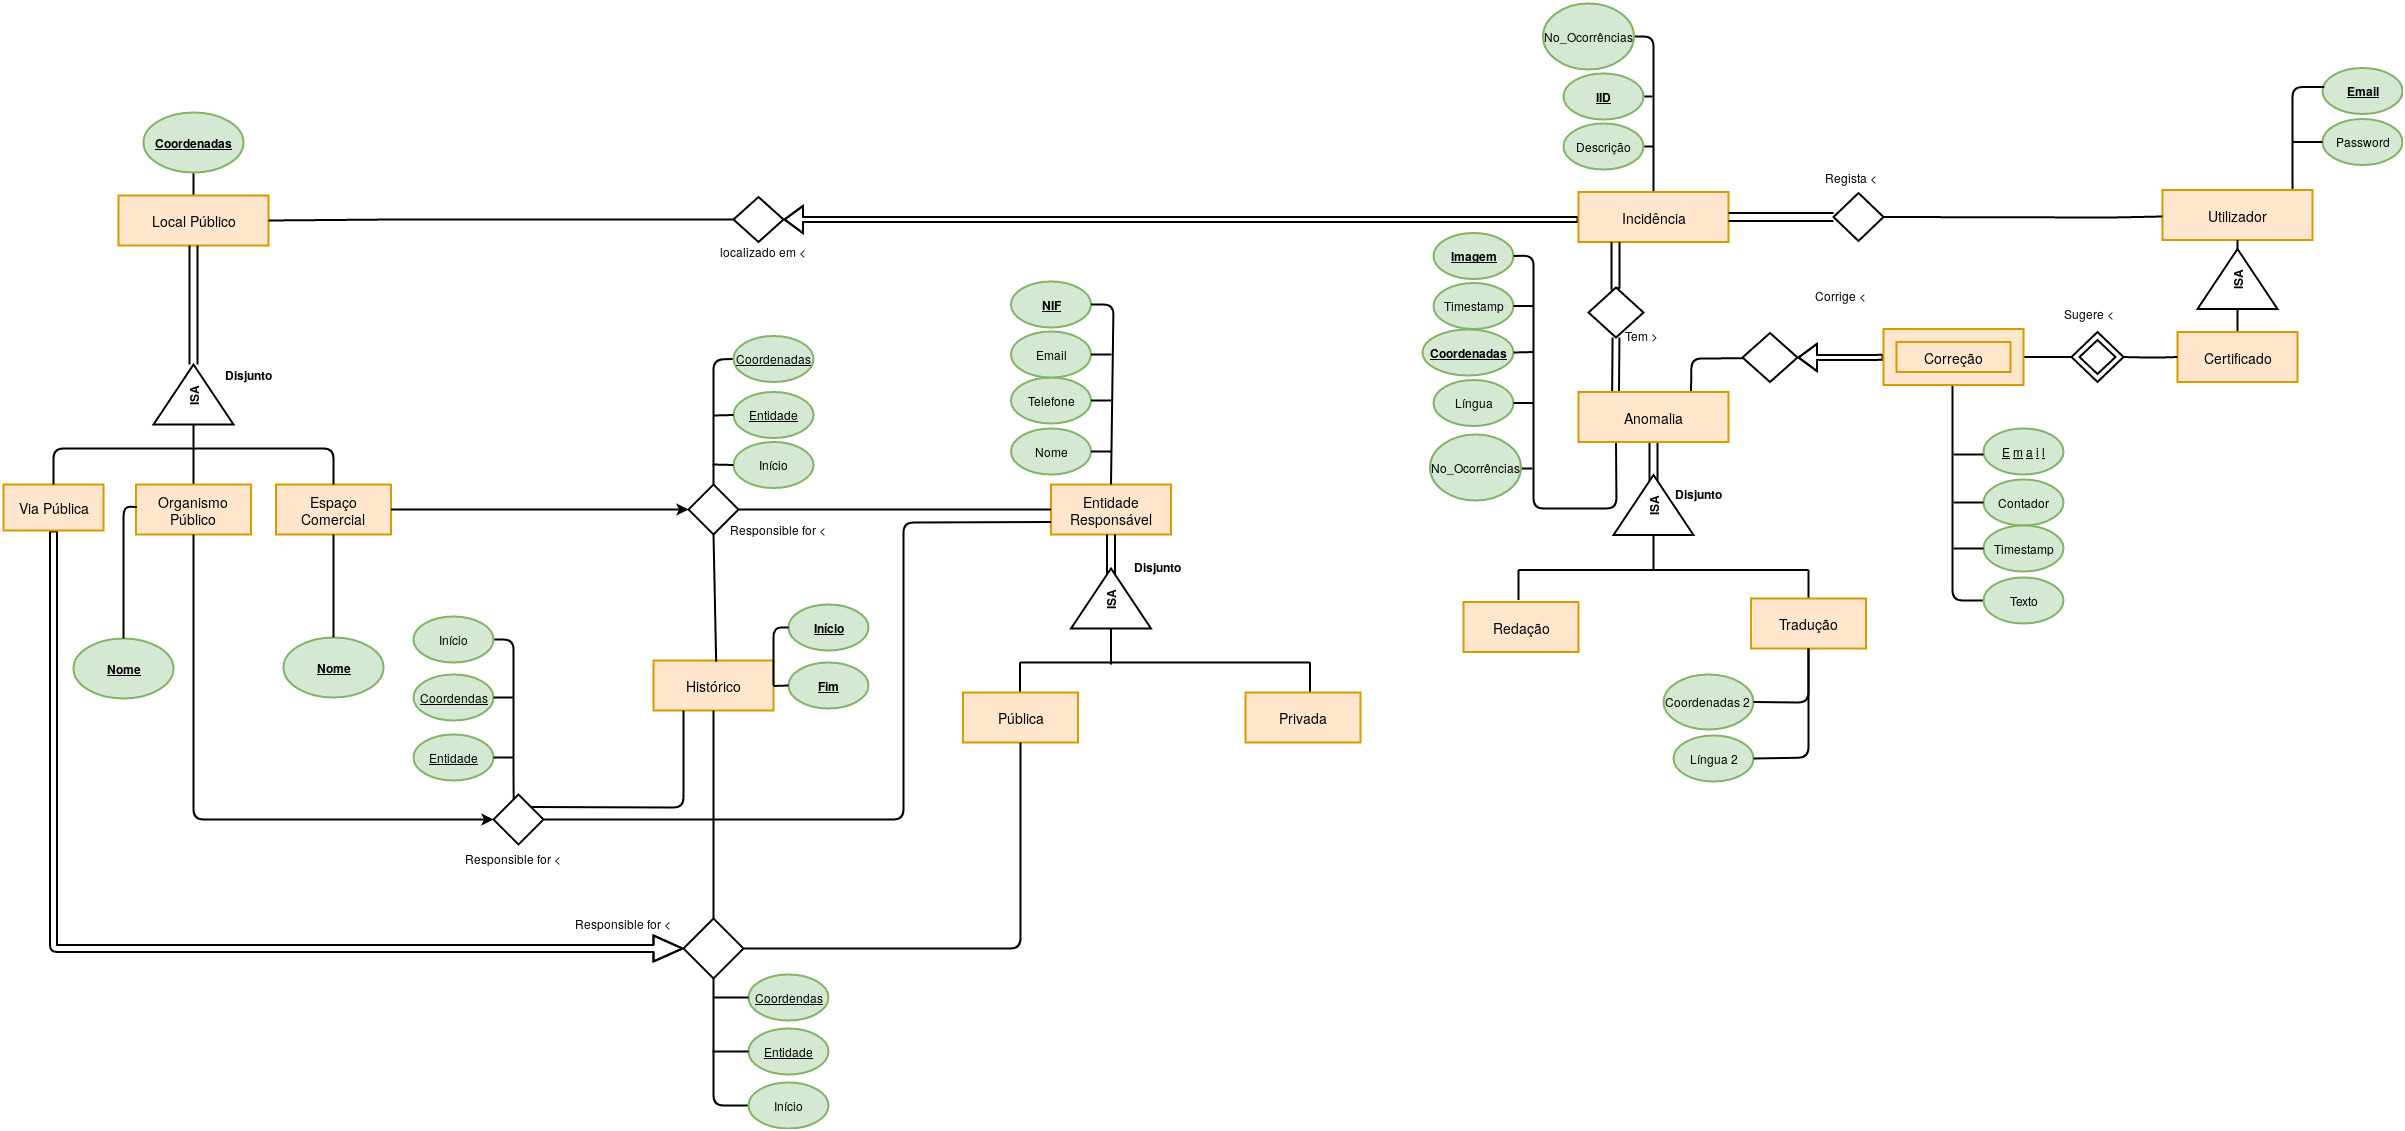
\includegraphics[width=1.4\textwidth, angle=90]{BDProj1.jpg}
\end{center}
\newpage

    \LARGE
    \begin{center}
        \textbf{Problemas do Modelo e Restrições de Integridade}
    \end{center}

    \bigskip
    \bigskip

    \normalsize

    \noindent De seguida apresentam-se as justifações às decisões tomadas durante a conceção do modelo. 

    \vspace*{10mm}
    \noindent\textbf{INCIDÊNCIA}

        As incidências foram consideradas como entidades independentes. Deste modo, são-lhes atribuídos IDs para as identificar.
        Dado que uma incidência se refere a anomalias, considerou-se que a primeira não pode existir sem ter uma anomalia, nem estar associada a nenhum local.
    
    \vspace*{10mm}
    \noindent\textbf{ANOMALIA}

        
        Uma anomalia é identificada pela zona da imagem que a caracteriza, sendo a imagem e a respetiva zona atributos distintos.
        Uma anomalia pode pertencer a várias incidências (permite identificar anomalias duplicadas).
        O modelo não proíbe que uma anomalia de tradução tenha zonas de imagens ou par de línguas iguais. Serão impostas restrições de integridade para que as duas zonas não se sobreponham e as línguas não sejam iguais.
    
    \vspace*{10mm}
    \noindent\textbf{CORREÇÃO}

        
        Uma correção é tomada como uma entidade fraca uma vez que esta não existe sem um utilizador que a crie nem uma anomalia para corrigir. Estes são precisos para a identificar.
    

    \vspace*{10mm}
    \noindent\textbf{HISTÓRICO}

        
        O Histórico foi modelado como uma entidade independente, com os seus próprios atributos e métodos, associada aos locais e Entidades Responsáveis para permitir que uma entidade seja responsável pelo mesmo local em períodos de tempo distintos.
        O Histórico tem a data de início e de fim dos períodos de responsabilidade para permitir que uma entidade responsável seja responsável por um mesmo local em períodos distintos. A data de fim não pode ser anterior à data de início.
    

    \vspace*{10mm}
    \noindent\textbf{ENTIDADES}

        
        O organismo público e o espaço comercial têm cada um o seu atributo primário ("nome"). Será imposta uma restrição de integridade para que os 
        nomes destes não sejam iguais. Esta unicidade do nome poderia ser resolvida com uma associação das duas entidades a uma super-entidade, 
        mas tal não seria coerente com os conceitos desenvolvidos no presente modelo. Para além disso, também não permitiria que, 
        futuramente, um organismo público e um espaço comercial venham a ter o mesmo nome.
    

\end{document}